\newpage
\section{Binomial Convolution Curvature Estimator}

Binomial Convolution Curvature Estimator (BCC) is an algorithm that calculate the curvature of a contour, by using a discrete convolution product. \newline
The algorithm of Malgouyres et al. use derivative Kernel \& smoothing Kernel \cite{malgouyres2008binomial}

\subsection{Smoothing Kernel}
The author give a smoothing kernel defined like that:


\[ h_{n}(x) = \left\{ 
  \begin{array}{l l}
    \begin{array}{c}
      n \\
      a + \frac{n}{2}
    \end{array} & \quad \text{if $n$ is even}\\
    \begin{array}{c}
      n \\
      a + \frac{n+1}{2}
    \end{array}& \quad \text{if $n$ is odd}\\
    0 & otherwise
  \end{array} \right.\]

 \subsection{Derivative Kernel}
 The derivative kernel is defined by the function:

	\begin{align*}
	B_{n}(a) = \delta * H_{n}(a) 
	\end{align*}

where $ \delta $ is defined by the function:

\[ \delta(x) = \left\{ 
  \begin{array}{l l}
  1 & \quad \text{if $x$ = 0}\\
  -1 & \quad \text{if $x$ = 1}\\
  0 & otherwise
  \end{array} \right.\]
\subsection{Calcul of the curvature}
 To calculate the curvature, we compute

 \begin{align*}
	Curvature =  \frac{ D_{n}^2(x) * D_{n}(y)  -  D_{n}^2(y) * D_{n}(x) }{D_{n}^2(x) + D_{n}^2(y)}
 \end{align*}
Where
  \begin{align*}
	n = h^{2(\alpha - 3)/3}
  \end{align*}

$ h $ Represent the grid size. When we compute the algorithm, we increase the grid size on every step.

\subsection{Implementation}\FloatBarrier
To implement this algorithm, we used the libraryr DGtal to get access to differents objects and functions. We tried to implement the same algorithm to be computed on the GPU (Parallel) but we had some difficulties to work with the source code of the DGtal library that is fully written in a generic style. We tried to use CUDA and openCL but we didn't get the algorithm working in parallel. In fact we could put some calculs in parallel, but it's not really usefull to put only one addition or multiplication in parallel. That's why we focused on the full algorithm in parallel.

\begin{figure}[h]
    \centering
    \subfloat[Source File]{{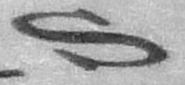
\includegraphics[width=5cm]{project/images/bcc_source.png} }}
    \qquad
    \subfloat[Result after applying the algorithm]{{
\includegraphics[width=5cm]{project/images/bcc_result.png} }}
    \caption{Source and Result}
    \label{fig:example}
\end{figure}

\subsection{Usage}
For testing this algorithm, go to the folder \textbf{TestBCC}, execute \textbf{cmake}, then \textbf{make}. Then run :\\
./main -f ../images/contourS.fc --gridStepInit 0.001 --gridStepIncrement  0.0005 --gridStepFinal 0.05 -o result.ppm \\
